Aktivierungsfunktionen ermöglichen den Neuronen nicht-lineare Outputs zu produzieren. Außerdem wird durch diese Funktionen entschieden, 
welche Neuronen aktiviert werden und wie die Inputs gewichtet werden. Zur Notation von Aktivierungsfunktion nutzen wir $\Phi$.
$$\hat{y} = \Phi(\overline{W} \cdot \overline{X})$$
\paragraph{Lineare Aktivierung}
Die simpelste Aktivierungsfunktion $\Phi(\cdot)$ ist die lineare Aktivierung. Sie bietet keine nicht linearität. Sie wird oft in Output Nodes
verwendet, wenn das Ziel ein reeller Wert ist \cite{CA18}.
$$\Phi(v) = v$$
\paragraph{Nicht lineare Aktivierung}
Um auch nicht lineare Probleme lösen zu können, werden nicht lineare Aktivierungsfunktionen verwendet. In den frühen Tagen der Entwicklung von neuralen Netzen wurden sign, sigmoid und hyperbolic tangent Funktionen genutzt.
Die sign Funktion $\Phi(v) = \text{sign}(v)$ generiert nur binäre \{-1,+1\} Ausgaben. Aufgrund der Nichtstetigkeit der Funktion, können beim Trainieren keine Loss-Funktionen verwendet werden.
Die Sigmoid Funktion $\Phi(v) = \frac{1}{1 + e^{-v}}$ generiert Werte zwischen 0 und 1. Sie eignet sich deshalb für Rechnungen die als Wahrscheinlichkeiten interpetiert werden sollen.
Der Graph der Tanh Funktion $\Phi(v) = \frac{e^{2v} - 1}{e^{2v} + 1}$ hat eine ähneliche Form wie die der Sigmoid Funktion. Sie unterscheidet sich jedoch in der Skalierung, denn ihr Wertebereich liegt zwischen -1 und 1.
Die Tanh Funktion lässt sich auch durch die Sigmoid Funktion darstellen \cite{CA18}.
$$\text{tanh}(v) = 2 \cdot \text{sigmoid}(2v) - 1$$
Wenn die Ausgabe der Berechnung postitiv sowie negativ sein kann, ist die tanh Funktion der sigmoid Funktion vorzuziehen. Außerdem ist es einfacher zu trainieren, weil die Funktion Mittelwertzentriert
und der Gradient größer ist \cite{CA18}.

\paragraph{Piecewise lineare Aktivierung}
Historisch wurden die Sigmoid und Tanh Funktion zur Einführung von Nichtliniearität genutzt. Heutzutage sind piecewise linear activation Funktionen (Stückweise Linear) beliebter, weil diese das Trainieren 
von mehrschichtigen neuronalen Netzen einfacher machen.
Zu den am häufigsten genutzten Aktivierungsfunktionen gehört ReLU (Rectified Linear Unit) $\Phi(v) = \text{max}\{v,0\}$. Das Ergebnis der ReLU Funktion ist 0, wenn die gewichtete Summe der Inputs $v$ kleiner 0 ist, sonst ist das Ergbenis das unveränderte $v$.
Eine weitere oft genutzte Aktivierungsfunktion ist die hard tanh Funktion $\Phi(v) = \text{max}\{\text{min}[v,1],-1\}$. Das Ergbenis der hard tanh Funktion ist -1 für $v < 1$ oder 1 für $v > 1$. Sonst ist das Ergbenis das unveränderte $v$ \cite{CA18}. 

\paragraph{Differenzierbarkeit von Aktivierungsfunktionen}
Die meisten neuralen Netze verwenden das Gradienten-Abstiegsverfahren zum Lernen. \cite{CA18} Aus diesem Grund ist die Differenzierbarkeit von Aktivierungsfunkionen besonders wichtig. Die Ableitung der linearen Aktivierungsfunktion ist immer 1.
Die Ableitung von $sign(v)$ ist 0 für alle Werte außer $v = 0$. Die fehlende Stetigkeit dieser Funktion ist einer der Gründe, weshalb diese selten in Verlustfunktionen verwendet wird, auch wenn sie als Aktivierungsfunktion verwendet wurde. 
Alle anderen vorher aufgezählten Aktivierungsfunktionen sind differenzierbar. \cite{CA18}

\begin{figure}[htbp]
    \centering
    \begin{subfigure}{0.3\textwidth}
      \centering
      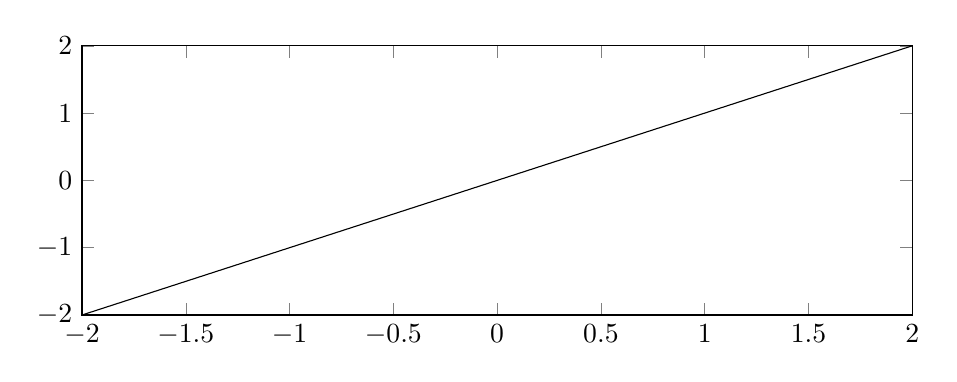
\begin{tikzpicture}
        \begin{axis}[
          width=\textwidth,
          height=5cm,
          xmin=-2,
          xmax=2,
          ymin=-2,
          ymax=2
        ]
          \addplot[black, domain=-2:2, samples=100] {x};
        \end{axis}
      \end{tikzpicture}
      \caption{Linear}
      \label{fig:plot1}
    \end{subfigure}
    \hfill
    \begin{subfigure}{0.3\textwidth}
        \centering
        \begin{tikzpicture}
          \begin{axis}[
            width=\textwidth,
            height=5cm,
            xmin=-2,
            xmax=2,
            ymin=-1.1,
            ymax=1.1,
            samples=100,
            xtick={-2,-1,0,1,2},
            ytick={-1,0,1},
            clip=false
          ]
            % Plot the sign function
            \addplot[black, thick, mark=none, domain=-2:0] {-1};
            \addplot[black, thick, mark=none, domain=0:2] {1};
            \draw (axis cs:0,-1) -- (axis cs:0,1);
          \end{axis}
        \end{tikzpicture}
        \caption{Sign Function}
        \label{fig:plot2}
      \end{subfigure}
    \hfill
    \begin{subfigure}{0.3\textwidth}
      \centering
      \begin{tikzpicture}
        \begin{axis}[
          width=\textwidth,
          height=5cm,
          xmin=-15,
          xmax=15,
          ymin=-1,
          ymax=1.1
        ]
          % Plot 3 data and settings
          \addplot[black, domain=-15:15, samples=100] {1/(1 + exp(-x))};
        \end{axis}
      \end{tikzpicture}
      \caption{Sigmoid}
      \label{fig:plot3}
    \end{subfigure}
  
    \medskip
  
    \begin{subfigure}{0.3\textwidth}
      \centering
      \begin{tikzpicture}
        \begin{axis}[
          width=\textwidth,
          height=5cm,
          xmin=-6.5,
          xmax=6.5,
          ymin=-1.1,
          ymax=1.1
        ]
          % Plot 4 data and settings
          \addplot[black, domain=-6.5:6.5, samples=100] {(exp(2*x)-1)/(exp(2*x)+1)};
        \end{axis}
      \end{tikzpicture}
      \caption{Tanh}
      \label{fig:plot4}
    \end{subfigure}
    \hfill
    \begin{subfigure}{0.3\textwidth}
      \centering
      \begin{tikzpicture}
        \begin{axis}[
            width=\textwidth,
            height=5cm,
            xmin=-2,
            xmax=2,
            ymin=-1.1,
            ymax=1.1
        ]
          % Plot 5 data and settings
          \addplot[black, domain=-2:2, samples=100] {max(x,0)};
        \end{axis}
      \end{tikzpicture}
      \caption{ReLU}
      \label{fig:plot5}
    \end{subfigure}
    \hfill
    \begin{subfigure}{0.3\textwidth}
      \centering
      \begin{tikzpicture}
        \begin{axis}[
            width=\textwidth,
            height=5cm,
            xmin=-2,
            xmax=2,
            ymin=-1.1,
            ymax=1.1
        ]
          % Plot 6 data and settings
          \addplot[black, domain=-2:2, samples=100] {max(min(x,1),-1)};
        \end{axis}
      \end{tikzpicture}
      \caption{Hard Tanh}
      \label{fig:plot6}
    \end{subfigure}
  
    \caption{Aktivierungsfunktionen}
    \label{fig:grid}
  \end{figure}
  